\begin{center}
	{\Large\bf 单元测验:重积分}
	
	(时间:150分钟)
\end{center}

{\bf 一、填空题(每题3分)}

\bigskip

1.\;$\ds\iint\limits_{|x|+|y|\leq 1}(|x|+y)\d\sigma=$\underline{\hspace{4cm}}

2.\;区域$D$由$x=y=0,x+y=1$所围成,且$\dint_0^1f(x)\d x=\dint_0^1xf(x)\d x$,
则

$\ds\iint\limits_Df(x)\d\sigma=$\underline{\hspace{4cm}}

3.\;设$I=\dint_0^1\dint_{e^x}^{e^{2x}}f(x,y)\d y\d x$,交换积分次序后
$I=$\underline{\hspace{6cm}}

\bigskip

4.\;$\dint_0^1\dint_0^{1+\sqrt{1-x^2}}f(x,y)\d y\d x$化为极坐标下的累次积分
(先积$\rho$)为\underline{\hspace{4cm}}

\bigskip

5.\;$\dint_0^1\dint_{-\sqrt{y-y^2}}^{\sqrt{y-y^2}}
\dint_0^{\sqrt{3(x^2+3y^2)}}f\left(
\sqrt{x^2+y^2+z^2}\right)\d z\d x\d y$化为柱坐标下的积分(先积$z$)为

\bigskip\bigskip

\underline{\hspace{8cm}}

\bigskip

{\bf 二、选择题(每题3分)}

\bigskip

1.\;设区域$D$由$x\geq 0,y\geq0$和$x+y=\df14,x+y=1$所围,
则以下积分满足(\underline{\hspace{1cm}})
$$I_1=\iint\limits_D[\ln(x+y)]^3\d\sigma,\quad
I_2=\iint\limits_D(x+y)^3\d\sigma,\quad
I_3=\iint\limits_D[\sin(x+y)]^3\d\sigma$$

  \quad(A)$I_1<I_2<I_3$\hspace{1cm}(B)$I_3<I_2<I_1$\hspace{1cm}
  (C)$I_1<I_3<I_2$\hspace{1cm}(D)$I_3<I_1<I_2$

\bigskip

2.\;设$a,b>0$,则$\ds\iint\limits_{\frac{x^2}{a^2}+\frac{y^2}{b^2}\leq1}
\sqrt{1-\df{x^2}{a^2}-\df{y^2}{b^2}}\d\sigma=$(\underline{\hspace{1cm}})
%   \ps{D}
  
  \quad(A)$\df23\pi ab$\hspace{1cm}(B)$\df43\pi ab$\hspace{1cm}
  (C)$\df23\pi a^2b^2$\hspace{1cm}(D)$\df43\pi a^2b^2$
  
\bigskip
  
3.\;设$\Omega:z\geq{\sqrt{x^2+y^2}},1\leq z\leq 2$则  
  $\ds\iiint\limits_{\Omega}f(x^2+y^2+z^2)\d V=$
  (\underline{\hspace{1cm}})
%   \ps{A}
  \begin{enumerate}[(A)]
    \setlength{\itemindent}{1cm}
    \item $\dint_1^2\dint_0^{2\pi}\dint_0^zf(r^2+z^2)r\d r\d\theta\d z$
    \item $\dint_0^{2\pi}\dint_1^2r\dint_0^1f(r^2+z^2)\d z\d r\d\theta$
    \item $\dint_0^{2\pi}\dint_0^{\frac{\pi}4}\dint_1^2
    f(r^2)r^2\sin\varphi\d r\d\varphi\d\theta$
    \item $\dint_0^{2\pi}\dint_{\frac{\pi}2}^{\frac{\pi}4}\dint_1^2
    f(r^2)r^2\sin\varphi\d r\d\varphi\d\theta$
  \end{enumerate}

\bigskip

4.\;设$f(x)$可微,$f(0)=1$,则$\lim\limits_{t\to0^+}\df1{\pi t^3}
  \ds\iint\limits_{x^2+y^2\leq t^2}  f(\sqrt{x^2+y^2})\d x\d y=$ 
  (\underline{\hspace{1cm}})
%   \ps{C}
  
  \quad(A)$0$\hspace{1cm}(B)$\df23f'(0)$\hspace{1cm}
  (C)$+\infty$\hspace{1cm}(D)不存在但也不是$\infty$

\bigskip

% 5.\;设$f(x,y)$连续,则$\dint_0^1\d x\dint_{-\sqrt{1-y^2}}^{1-y}f(x,y)\d y=$
%   (\underline{\hspace{1cm}})
% %   \ps{D}
%   \begin{enumerate}[(A)]
%     \setlength{\itemindent}{1cm}
%     \item $\dint_0^1\d x\dint_{0}^{x-1}f(x,y)\d y
%     +\dint_{-1}^0\d x\dint_0^{\sqrt{1-x^2}}f(x,y)\d y$
%     \item $\dint_0^1\d x\dint_{0}^{1-x}f(x,y)\d y
%     +\dint_{-1}^0\d x\dint_{-\sqrt{1-x^2}}^0f(x,y)\d y$
%     \item $\dint_0^{\frac{\pi}2}\d\theta\dint_0^{\frac1{\cos\theta+\sin\theta}}
%     f(r\cos\theta,r\sin\theta)\d r+\dint_{\frac{\pi}2}^{\pi}\d\theta
%     \dint_0^1f(r\cos\theta,r\sin\theta)\d r$
%     \item $\dint_0^{\frac{\pi}2}\d\theta\dint_0^{\frac1{\cos\theta+\sin\theta}}
%     f(r\cos\theta,r\sin\theta)r\d r+\dint_{\frac{\pi}2}^{\pi}\d\theta
%     \dint_0^1f(r\cos\theta,r\sin\theta)r\d r$
%   \end{enumerate}

5.\;$\ds\iint\limits_{x^4+y^4\leq1}\df{x^2+xy-y^2}{x^2+y^2}\d\sigma=$
(\underline{\hspace{1cm}})

  \quad(A)$\df12$\hspace{1cm}(B)$\pi$\hspace{1cm}
  (C)$\df{\pi}2$\hspace{1cm}(D)以上都不对

{\bf 三、}(6分)计算二重积分$\ds\iint\limits_D\ln\sqrt{x^2+y^2}\d\sigma$,其中$D:1\leq
x^2+y^2\leq e^2$

\bigskip

{\bf 四、}(6分)设$f(z)$连续,证明:
$$\iiint\limits_{x^2+y^2+z^2\leq 1}f(z)\d V=\pi\dint_{-1}^1f(u)(1-u^2)\d u$$

\bigskip

% {\bf 五、}(6分)计算$\dint_0^4\dint_{\sqrt x}^{\mathrm{min}\{x,2\}}\sin\df{x}{2y}\d
% y\d x$

{\bf 五、}(6分)
% 改变如下累次积分的积分次序
% $$\dint_0^4\dint_{\sqrt x}^{\mathrm{min}\{x,2\}}
% 	\sin\df{x}{y}\d y\d x$$
改变以下累次积分的积分次序
$$\dint_0^4\dint_{\sqrt x}^xf(x,y)\d y\d x$$

\bigskip

{\bf 六、}(6分)求四条直线$x+y=p,\,x+y=q,\,y=ax,\,y=bx$($0<p<q,\,0<a<b$)所围成的图形面积。

\bigskip

{\bf 七、}(6分)将三次积分$\dint_0^2\dint_0^{\sqrt{2x-x^2}}\dint_0
^{\sqrt{x^2+z^2}}y\sqrt{x^2+z^2}\d
y\d z\d x$化为柱坐标下的三次积分,并求其值。

\bigskip

{\bf 八、}(8分)设$a>0$,$D_1$为第一象限内由$x$轴及$x^2+y^2=a^2,\,x^2-2ax+y^2=0$所围成的区域,求
$\ds\iint\limits_{D_1}\sqrt{x^2+y^2}\d\sigma$


\bigskip

{\bf 九、}(8分)
% 设$h=\sqrt{x^2+y^2+z^2}$,$[h]$表示不大于$h$
% 的最大整数,计算极限
% $$\lim\limits_{n\to\infty}\df 1{n^4}\iiint\limits_{h\leq n}[h]\d V$$
设$\Omega=\{\;x^2+y^2+(z-1)^2\leq1,\;z\geq 1,\;y\geq 0\}$,求
$$\iiint\limits_{\Omega}\df{\d V}{\sqrt{x^2+y^2+z^2}}.$$

\bigskip

% {\bf 十、}(8分)计算积分
% $$\dint_0^1\dint_0^{1-x}\dint_0^{1-z-x}(1-y)e^{-(1-y-z)^2}\d y\d z\d x$$

{\bf 十、}(10分)设$\Omega:\df{x^2}{a^2}+\df{y^2}{b^2}+\df{z^2}{c^2}\leq 1$,
计算积分
$$\iiint\limits_{\Omega}(x+y-2z)^2\d V$$

\bigskip

{\bf 十一、}(6分)求$I=\ds\iiint\limits_{\Omega}(x+y)\d V$,其中$\Omega$由$x=0,x=1$和
$x^2+1=y^2+z^2$所围成。

\bigskip

{\bf 十二、}(8分)一个底半径为$R$,高为$H$的圆锥体,在其地面上拼接一个半径为$R$的半球,假设
该立体的密度均匀,要使其形心恰好落在球心上,问$R$和$H$需要满足什么关系?

\newpage

\begin{center}
	{\Large\bf 解答与评分标准}\ps{\b 
	1.若解法与参考答案不同,参照本评分标准的特点分段给分\\
	2.计算题只写结果,缺少计算过程,最多得1分}
\end{center}

{\bf 一、填空题(每题3分)}

1.\;[提示]:由对称性$\iint\limits_{|x|+|y|\leq 1}y\d\sigma=0$,故
$$\mbox{原式}=4\dint_0^1\dint_0^{1-x}x\d y\d x=\ldots=\df23.$$

2.\;[提示]:
$$\mbox{原式}=4\dint_0^1\dint_0^{1-x}f(x)\d y\d x=\dint_0^1f(x)\d x
-\dint_0^1xf(x)\d x=0.$$

3.\;$\left(\dint_1^e\dint_{\frac{\ln y}2}^{\ln y}+
\dint_e^{e^2}\dint_{\frac{\ln y}2}^{1}\right)f(x,y)\d x\d y$

4.\;$\left(\dint_0^{\frac{\pi}4}\dint_0^{2\sin\theta}
+\dint_{\frac{\pi}4}^{\frac{\pi}2}\dint_0^{\frac1{\cos\theta}}\right)
f(\rho\cos\theta,\rho\sin\theta)\rho\d\rho\d\theta$

5.\;$\dint_{-\frac{\pi}2}^{\frac{\pi}2}\dint_0^{\sin\theta}
\dint_0^{\rho\sqrt{3(1+2\sin^2\theta)}}f(\rho)\rho\d z\d\rho\d\theta$

{\bf 二、选择题(每题3分)}

1.\;C. 

[提示]:在区域$D$内,$\ln(x+y)\leq0<\sin(x+y)\leq x+y$

2.\;A.

[提示]:该积分等于上半椭球$\df{x^2}{a^2}+\df{y^2}{b^2}+z^2=1\;(z\geq
0)$的体积,也即$\df23\pi ab$。
\ps{椭球$\df{x^2}{a^2}+\df{y^2}{b^2}+\df{z^2}{c^2}=1$的体积为$\df43\pi abc$}

3.\;A.

4.\;C.

[提示]:
\begin{align*}
	\mbox{原式}&=\lim\limits_{t\to0^+}\df1{\pi t^3}
	\dint_0^{2\pi}\dint_0^tf(\rho)\rho\d\rho\d\theta\\
	&=\lim\limits_{t\to0^+}\df{2\pi f(t)t}{3\pi t^2}
	=\lim\limits_{t\to0^+}\df{2f(t)}{3t}
\end{align*}
注意到以上极限内,分子分母分别趋于$1$和$0^+$,故结果为$+\infty$

5.\;D.

[提示]:由于积分区域关于$x=0$对称,$\df{xy}{x^2+y^2}$为关于$x$的偶函数,故
$$\iint\limits_{x^4+y^4\leq 1}\df{xy}{x^2+y^2}\d\sigma=0\quad
\Rightarrow\quad
\mbox{原式}=\iint\limits_{x^4+y^4\leq 1}\df{x^2-y^2}{x^2+y^2}\d\sigma.$$

又在积分区域中$x,y$可交换,故交换$x,y$积分值不变,从而
$$\mbox{原式}=\df12\left[\iint\limits_{x^4+y^4\leq
1}\df{x^2-y^2}{x^2+y^2}\d\sigma
+\iint\limits_{x^4+y^4\leq
1}\df{y^2-x^2}{y^2+x^2}\d\sigma\right]=0$$

{\bf 三、}(6分)[解]:令$x=\rho\cos\theta,y=\rho\sin\theta$,则
$$D:\;0\leq\theta\leq2\pi,\;1\leq\rho\leq e,\eqno{(+2\mbox{分})}$$
故
\begin{align*}
	\mbox{原式}&=\dint_0^{2\pi}\dint_1^e\rho\ln\rho\d\rho\d\theta\tag{+2分}\\
	&=\pi\dint_1^e\ln\rho\d\rho^2
	=\pi\left[\rho^2\ln\rho|_1^e-\dint_1^e\rho\d\rho\right]
	=\df{\pi}2(e^2+1)\tag{+2分}
\end{align*}

{\bf 四、}(6分)[证]:左端积分的积分区域可表示为
$$\Omega:\;-1\leq z\leq1,\;(x,y)\in D(z),\eqno{(+2\mbox{分})}$$
其中
$$D(z):\;x^2+y^2\leq 1-z^2,$$
其面积为$\ds\iint\limits_{D(z)}\d\sigma_{xy}=\pi(1-z^2)$,故
\hfill (+2分)
\begin{align*}
	\mbox{左边}&=\dint_0^1\iint\limits_{D(z)}f(z)\d\sigma_{xy}\d z
	=\dint_0^1f(z)\iint\limits_{D(z)}\d\sigma_{xy}\d z\\
	&=\dint_0^1f(z)\pi(1-z^2)\d z=\mbox{右边}\tag{+2分}
\end{align*}

{\bf 五、}(6分)[解]:如图
\begin{center}
	\resizebox{!}{6.5cm}{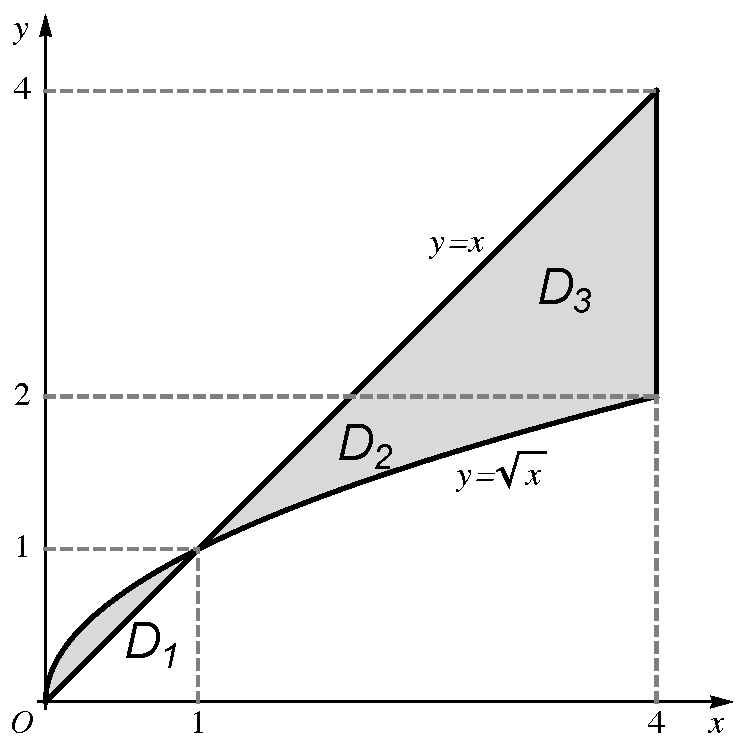
\includegraphics{./images/ch11/xSx.pdf}} 
\end{center}
$$\mbox{原式}=\left(-\iint\limits_{D_1}+\iint\limits_{D_2}
+\iint\limits_{D_3}\right)f(x,y)\d\sigma\eqno{(+3\mbox{分})}$$
其中
\begin{align*}
	D_1:&\;0\leq y\leq 1,\;y^2\leq x\leq y\\
	D_2:&\;1\leq y\leq 2,\;y\leq x\leq y^2\\
	D_3:&\;2\leq y\leq 4,\;y\leq x\leq 4
\end{align*}
故改变积分次序后
$$\mbox{原式}=\left(-\dint_0^1\dint_{y^2}^y
+\dint_1^2\dint_y^{y^2}+\dint_2^4\dint_y^4
\right)f(x,y)\d x\d y\eqno{(+3\mbox{分})}$$

{\bf 六、}(6分)[解]:令$u=x+y,v=\df yx$,则所述平面区域可表示为
$$D:\;p\leq u\leq q,\;a\leq v\leq b,\eqno{(+2\mbox{分})}$$
且
$$\left|\df{\p(u,v)}{\p(x,y)}\right|=\df{(v+1)^2}u.\eqno{(+2\mbox{分})}$$
故所求面积为
$$S=\dint_p^q\dint_a^b\df{u}{(v+1)^2}\d v\d u
=\df12(q^2-p^2)\left(\df1{a+1}-\df1{b+1}\right)\eqno{(+2\mbox{分})}$$

{\bf 七、}(6分)[解]:(图略)令
$$x=\rho\cos\theta, y=y, z=\rho\sin\theta,\eqno{(+2\mbox{分})}$$
则积分区域可表示为
$$\Omega:\;0\leq\theta\leq\df{\pi}2,\;0\leq\rho\leq2\cos\theta,
0\leq y\leq\rho,\eqno{(+2\mbox{分})}$$
故
\begin{align*}
	\mbox{原式}&=\dint_{0}^{\frac{\pi}2}\dint_0^{2\cos\theta}
	\dint_0^{\rho}y\rho^2\d y\d\rho\d\theta
	=\df12\dint_{0}^{\frac{\pi}2}\dint_0^{2\cos\theta}
	\rho^4\d\rho\d\theta\\
	&=\df{16}5\dint_0^{\frac{\pi}2}\cos^5\theta\d\theta
	=\df{16}5\dint_0^{\frac{\pi}2}(1-\sin^2\theta)^2\d\sin\theta=\df{128}{75}\tag{+2分}
\end{align*}

{\bf 八、}(8分)[解]:如图
\begin{center}
	\resizebox{!}{4cm}{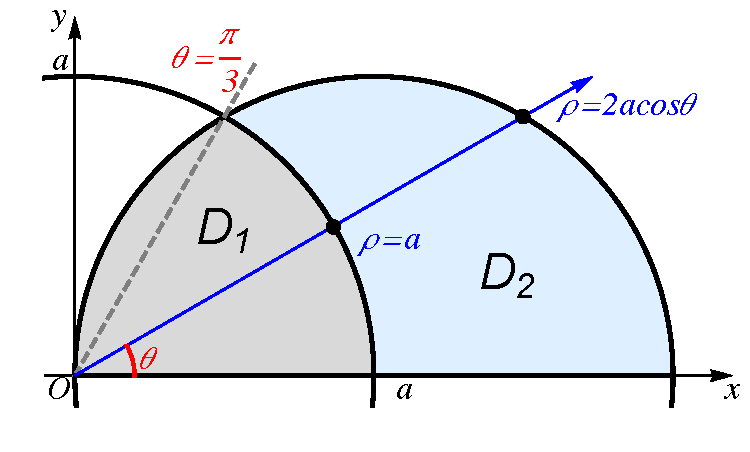
\includegraphics{./images/ch11/halfCircle-1.pdf}} 
\end{center}
$$\mbox{原式}=\left(\iint\limits_{D_1+D_2}-\iint\limits_{D_2}\right)
\sqrt{x^2+y^2}\d\sigma,$$
其中区域
$$D_1+D_2:\;0\leq\theta\leq\df{\pi}2,\;0\leq\rho\leq2a\cos\theta,\eqno{(+2\mbox{分})}$$
$$D_2:\;0\leq\theta\leq\df{\pi}3,\;a\leq\rho\leq2a\cos\theta,\eqno{(+2\mbox{分})}$$
故
\begin{align*}
	\mbox{原式}&=\dint_0^{\frac{\pi}2}\dint_0^{2a\cos\theta}\rho^2\d\rho\d\theta
	-\dint_0^{\frac{\pi}3}\dint_a^{2a\cos\theta}\rho^2\d\rho\d\theta\\
	&=\df13\dint_0^{\frac{\pi}2}8a^3\cos^3\theta\d\theta
	-\df13\dint_0^{\frac{\pi}3}(8a^3\cos^3\theta-a^3)\d\theta\\
	&=\df{8a^3}3\dint_{\frac{\pi}3}^{\frac{\pi}2}\cos^3\theta\d\theta
	+\df{\pi a^3}9=\left(\df{16+\pi}{9}-\sqrt3\right)a^3\tag{+4分}
\end{align*}

{\bf 九、}(8分)[解]:如图
\begin{center}
	\resizebox{!}{6cm}{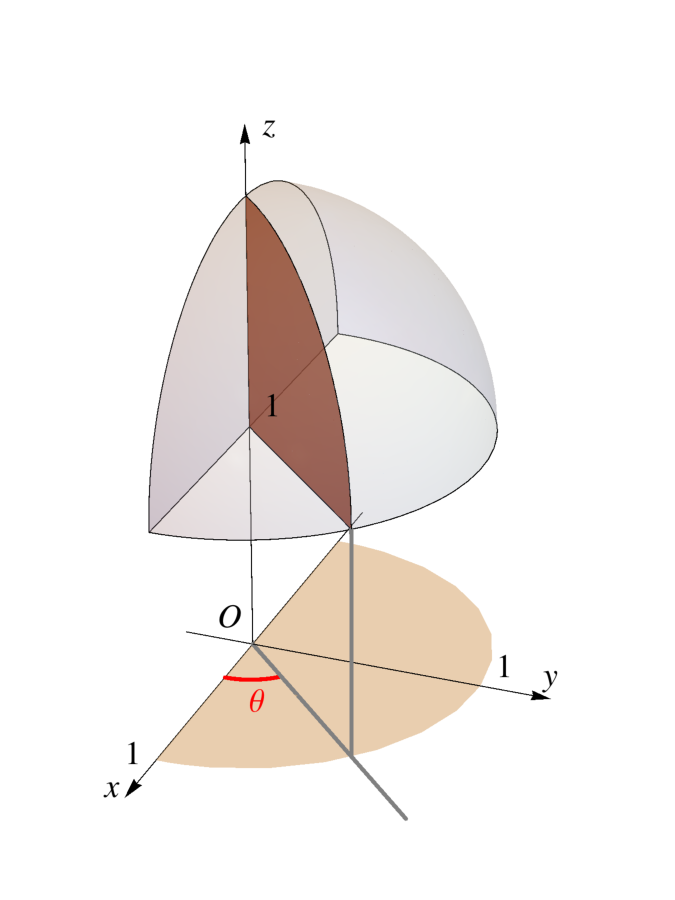
\includegraphics{./images/ch11/quaSphere-3D.pdf}}
	\quad\quad
	\resizebox{!}{6cm}{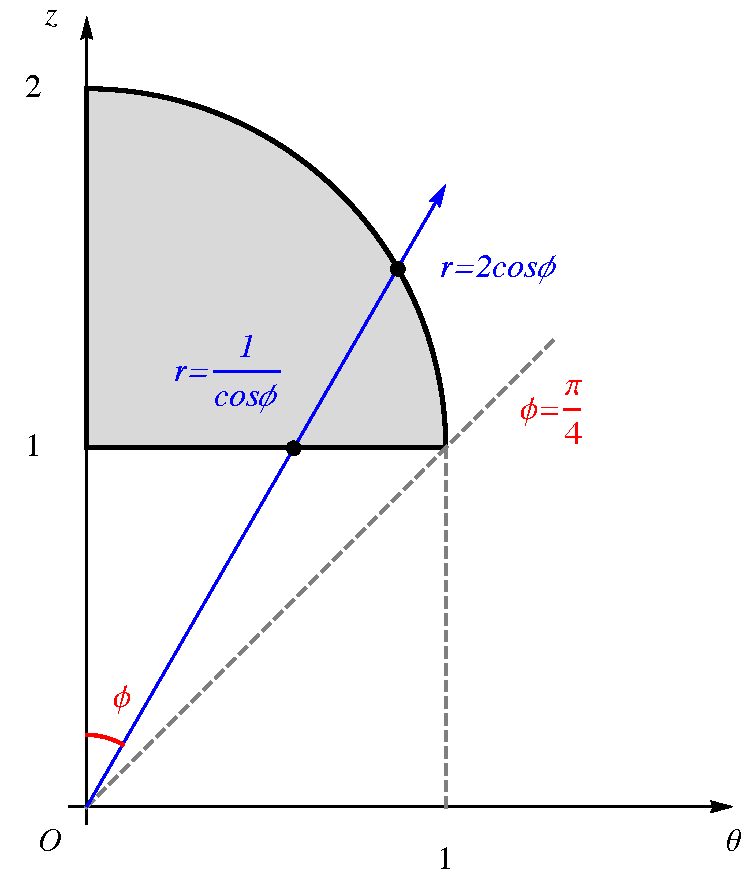
\includegraphics{./images/ch11/quaSphere-2D.pdf}} 
\end{center}
令$x=r\sin\phi\cos\theta,\;y=r\sin\phi\sin\theta,\;z=r\cos\phi$,则
$$\Omega:\;0\leq\theta\leq\pi,\;0\leq\phi\leq\df{\pi}4,\;
\df1{\cos\phi}\leq r\leq2\sin\phi,\eqno{(+4\mbox{分})}$$
故
\begin{align*}
	\mbox{原式}&=\dint_0^{\pi}\dint_0^{\frac{\pi}4}
	\dint_{\frac1{\cos\phi}}^{2\sin\phi}\df1rr^2\sin\phi
	\d r\d\phi\d\theta\\
	&=\df{\pi}2\dint_0^{\frac{\pi}4}\left(4\sin^2\phi-\df1{\cos^2\phi}\right)
	\sin\phi\d\phi=\df{\pi}6(11-8\sqrt2)\tag{+4分}
\end{align*}

{\bf 十、}(10分)[解]:(图略)注意到$\Omega$关于三个$x=0$对称,且$xy$为关于$x$的奇函数,故
$$\iiint\limits_{\Omega}xy\d V=0.$$
同理,
$$\iiint\limits_{\Omega}yz\d V=\iiint\limits_{\Omega}zx\d V=0.$$
从而
\begin{align*}
	\mbox{原式}&=\iiint\limits_{\Omega}(x^2+y^2+4z^2+2xy-4yz-4zx)\d V\\
	&=\iiint\limits_{\Omega}(x^2+y^2+4z^2)\d V\tag{+3分}
\end{align*}

又
$$\Omega:\;-c\leq z\leq c,\;(x,y)\in D(z),$$
其中$D(z):\;\df{x^2}{a^2}+\df{y^2}{b^2}=1-\df{z^2}{c^2}$面积为
$$\iint\limits_{D(z)}\d\sigma_{xy}=\pi ab\left(1-\df{z^2}{c^2}\right),$$
故
\begin{align*}
	\iiint\limits_{\Omega}z^2\d V
	&=\dint_{-c}^{c}\iint\limits_{D(z)}z^2\d\sigma_{xy}\d z
	=\dint_{-c}^{c}z^2\iint\limits_{D(z)}\d\sigma_{xy}\d z\\ 
	&=\dint_{-c}^{c}z^2\pi ab\left(1-\df{z^2}{c^2}\right)\d z
	=\df4{15}\pi abc^3. \tag{+3分}
\end{align*}

注意到在$\Omega$中$\df xa,\;\df yb,\;\df zc$可交换,故由轮换对称性可知
$$\iiint\limits_{\Omega}x^2\d V=\df4{15}\pi a^3bc,\quad
\iiint\limits_{\Omega}y^2\d V=\df4{15}\pi ab^3c.$$

综上,
$$\mbox{原式}=\df4{15}\pi abc(a^2+b^2+4c^2).\eqno{(+4\mbox{分})}$$

{\bf 十一、}(6分)[解]:(图略)注意到$\Omega$关于$y=0$对称\ps{用$-y$替换$y$,
$\Omega$不变},故
$$\iiint\limits_{\Omega}y\d V=0.\eqno{(+3\mbox{分})}$$

又
$$\Omega:\;0\leq x\leq 1,\;(y,z)\in D(x),$$
其中$D(x):y^2+z^2\leq x^2+1$的面积为
$$\iint\limits_{D(x)}\d\sigma_{yz}=\pi(x^2+1),$$
故
\begin{align*}
	\mbox{原式}&=\dint_0^1\iint\limits_{D(x)}x\d\sigma_{yz}\d x
	=\dint_0^1x\iint\limits_{D(x)}\d\sigma_{yz}\d x\\
	&=\dint_0^1x\pi(x^2+1)\d x=\df34\pi\tag{+3分}
\end{align*}

{\bf 十二、}(8分)[解]:如图
\begin{center}
	\resizebox{!}{6cm}{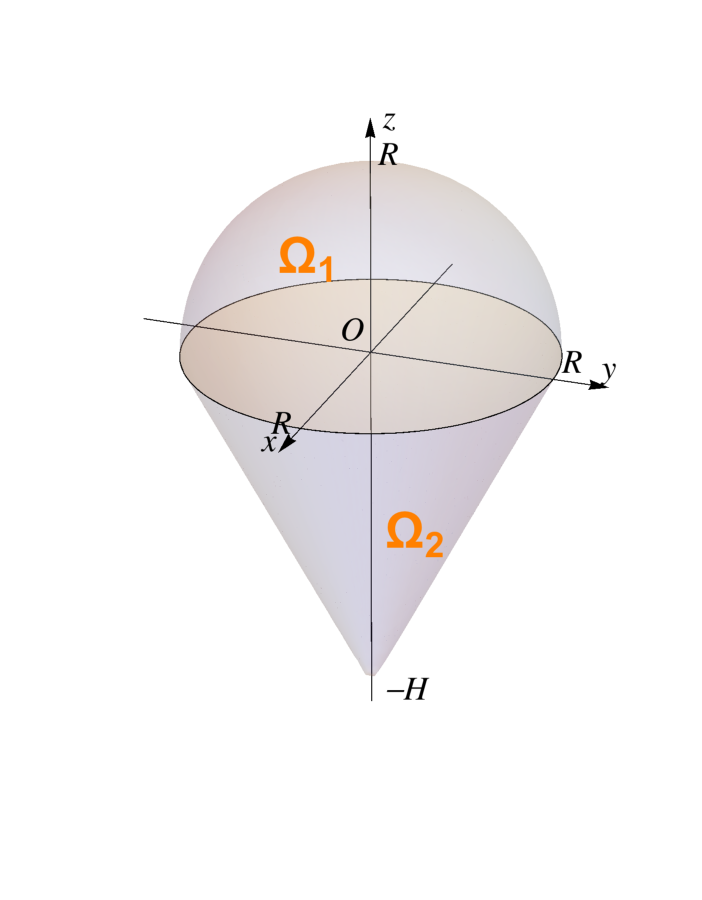
\includegraphics{./images/ch11/sAc.pdf}}
\end{center}
由题意,
$$\iiint\limits_{\Omega_1+\Omega_2}x\d V
=\iiint\limits_{\Omega_1+\Omega_2}y\d V
=\iiint\limits_{\Omega_1+\Omega_2}z\d V=0,$$
由对称性,前两个积分显然为零。\hfill (+2分)

以下分别在球坐标系和柱坐标系下计算$\ds\iiint\limits_{\Omega_1}z\d V$
和$\ds\iiint\limits_{\Omega_2}z\d V$。

$$
	\iiint\limits_{\Omega_1}z\d V=\dint_0^{2\pi}\dint_0^{\frac{\pi}2}
	\dint_0^Rr\cos\phi r^2\sin\phi\d
	r\d\phi\d\theta=\df{\pi}8R^4\eqno{(+3\mbox{分})} $$
$$
	\iiint\limits_{\Omega_2}z\d V=\dint_0^{2\pi}\dint_0^R
	\dint_{\frac{H}R(\rho-R)}^0\rho z\d z\d\rho\d\theta=-\df{\pi}{12} H^2R^2
$$
由$\ds\iiint\limits_{\Omega_1+\Omega_2}z\d V=0$,可得
$$\df23H^2=R^2,\eqno{(+3\mbox{分})}$$
即为所求。